\documentclass[10pt,a4paper]{article}
\usepackage[latin3]{inputenc}
\usepackage{amsmath}
\usepackage{amsfonts}
\usepackage{amssymb}
\usepackage{graphicx}
\author{Ricardo Arango - Big Bang Data}
\title{Modelo de Deserci�n en Clientes}
\begin{document}
\maketitle
	\noindent La fuga de clientes se define como el \textit{Movimiento de un cliente de un proveedor de servicio a otro}, mientras que la gesti�n de fuga de clientes describe el proceso por el cual el operador del servicio intenta evitar la fuga del cliente. En consecuencia, la utilizaci�n de modelos predictivos que permitan \textbf{identificar clientes en situaci�n de riesgo de fuga}, permite al operador dirigir esfuerzos en prevenir la salida del cliente.
	\section{Los Datos}
		La variable \textit{target} corresponde a la variable objetivo que se quiere predecir. En este caso, el abandono voluntario de clientes, esta variable es de car�cter booleano, \textbf{FALSE: cliente permanece con sus servicios � TRUE: clientes los abandona voluntariamente}.
		
		
		\begin{figure}[h]
			\centering
			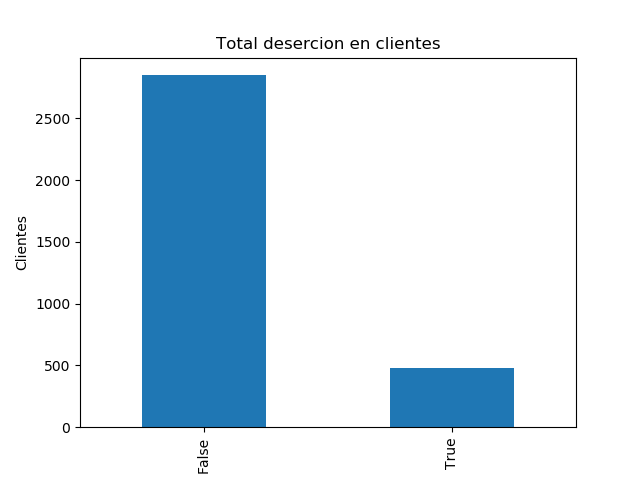
\includegraphics[width=0.5\textwidth]{count_churn}
		\end{figure}
		El $Odd_{desercion}=0.17$, es decir: por cada cliente que abandona los servicios, 6 clientes no lo hacen.
		\begin{equation*}
			Odd_{desercion}\approx\frac{1}{6}
		\end{equation*}
		La  meta es reducir dicho n�mero lo m�ximo posible aumentando, considerablemente, la cantidad de usuarios que permanecen con sus servicios.

		\vspace{0.5cm}
		A continuaci�n enumeraremos los rasgos m�s caracter�sticos presentes (hist�ricamente) en los  clientes que deciden abandonar los servicios. Esto con el fin de identificar posibles alarmas y evitar la fuga de cli

		\begin{figure}[h]
			\centering
			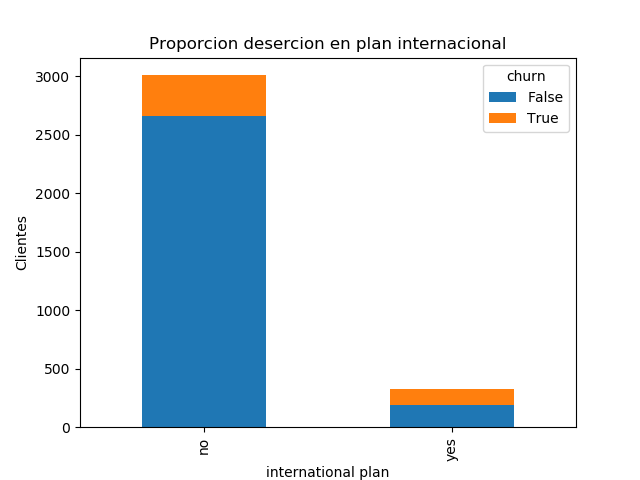
\includegraphics[width=0.5\textwidth]{prop_churn_inrternational}
		\end{figure}
		
		La medida del \textit{ratio} entre las variables de deserci�n y plan internacional es:
		\begin{equation*}
			ratio_{desercion,p-internacional} = 5.67
		\end{equation*}
		De dicho n�mero podemos inferir que la relaci�n entre estas dos variables es fuerte, es decir: \textbf{es muy probable que alguien con un plan internacional deserte}.
		\vspace{0.5cm}
		\begin{figure}[h]
			\centering
			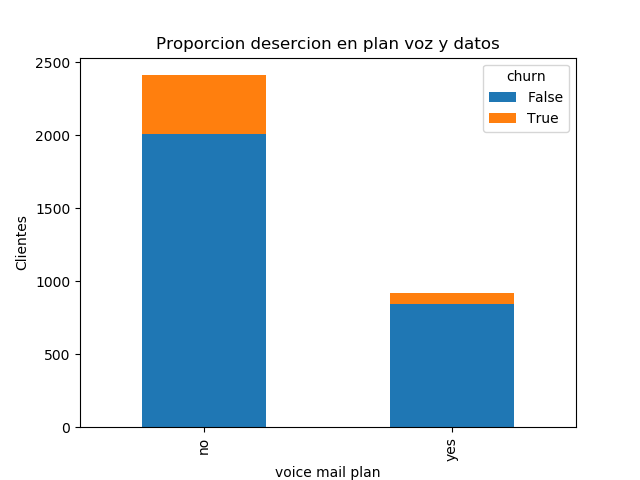
\includegraphics[width=0.5\textwidth]{prop_churn_voice_mail}
		\end{figure}
		
		La medida del \textit{ratio} entre las variables de deserci�n y plan de datos es:
		\begin{equation*}
		ratio_{desercion,p-datos} = 0.47
		\end{equation*}
		De dicho n�mero podemos inferir que la relaci�n entre estas dos variables es fuerte, es decir: \textbf{es muy probable que alguien con un plan de datos no deserte}.
		\vspace{0.5cm}
		
				
		\begin{figure}[h]
			\centering
			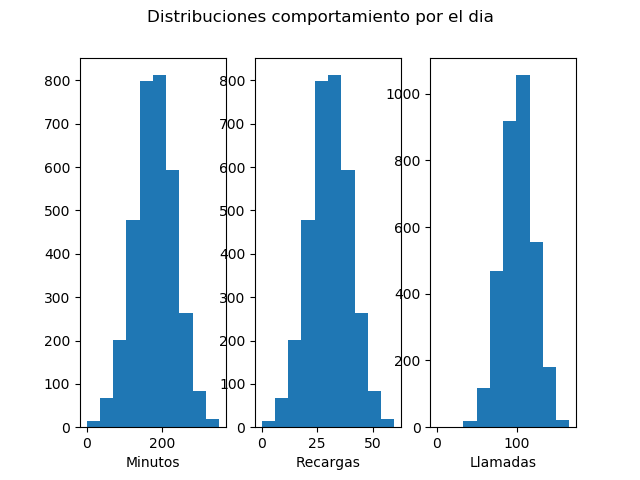
\includegraphics[width=0.5\textwidth]{cha_day}			
		\end{figure}
		De estas variables podemos inferir que el comportamiento \textbf{promedio} de un desertor en las horas de la ma�ana es:
		\begin{equation*}
			minutos=206 \ \ \ \  recargas=35 \ \ \ \ llamadas=101
		\end{equation*}
		\vspace{0.5cm}
		
		
		\begin{figure}[h]
			\centering
			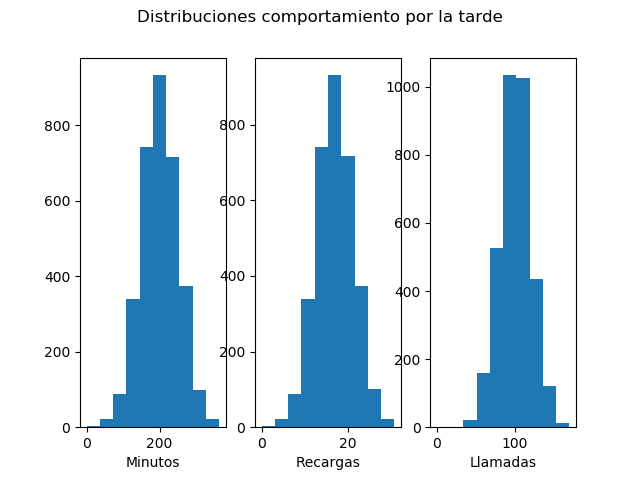
\includegraphics[width=0.5\textwidth]{cha_eve}			
		\end{figure}
		De estas variables podemos inferir que el comportamiento \textbf{promedio} de un desertor en las horas de la tarde es:
		\begin{equation*}
			minutos=212 \ \ \ \  recargas=18 \ \ \ \ llamadas=100
		\end{equation*}
		\vspace{0.5cm}
		
		
		\begin{figure}[h]
			\centering
			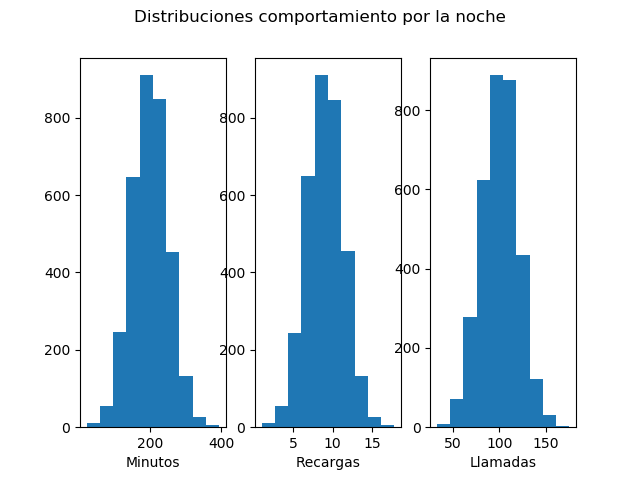
\includegraphics[width=0.5\textwidth]{cha_night}			
		\end{figure}
		De estas variables podemos inferir que el comportamiento \textbf{promedio} de un desertor en las horas de la noche es:
		\begin{equation*}
			minutos=205 \ \ \ \  recargas=9 \ \ \ \ llamadas=100
		\end{equation*}
	\newpage
	\section{El Modelo}
		  El problema de fuga de clientes ha sido objeto de una nutrida �rea de investigaci�n, tanto desde el punto de vista del marketing, enfoc�ndose en el comportamiento del consumidor y los componentes emocionales que la gatillan y desde el punto de vista de la miner�a de datos, enfoc�ndose en la aplicaci�n de algoritmos de machine learning para predecir el abandono de clientes. Del mismo modo, se han comparado diversos algoritmos para elaborar un puntaje de "propensi�n a la fuga" de clientes de telefon�a celular. Los �rboles de decisi�n y las regresiones log�sticas son los algoritmos que ofrecen la mejor precisi�n. La desventaja de este ultimo radica en que no es posible observar la cadena de condiciones que se deben cumplir para que un cliente tenga el potencial de abandonar el servicio. Dicho de otra forma, se trata de modelos de caja negra, en los cuales se hace dif�cil entender qu� es lo que gatilla o motiva una fuga.
		  \subsection{�rboles de Decisi�n}
		  	Los �rboles de decisi�n se definen como un procedimiento recursivo, en el cual un n�mero 'N' de registros se dividen progresivamente en grupos, de acuerdo a una regla de divisi�n que permita maximizar la homogeneidad o pureza de la variable \textit{target}.
		  	
		  	
  			\begin{figure}[h]
		  		\centering
		  		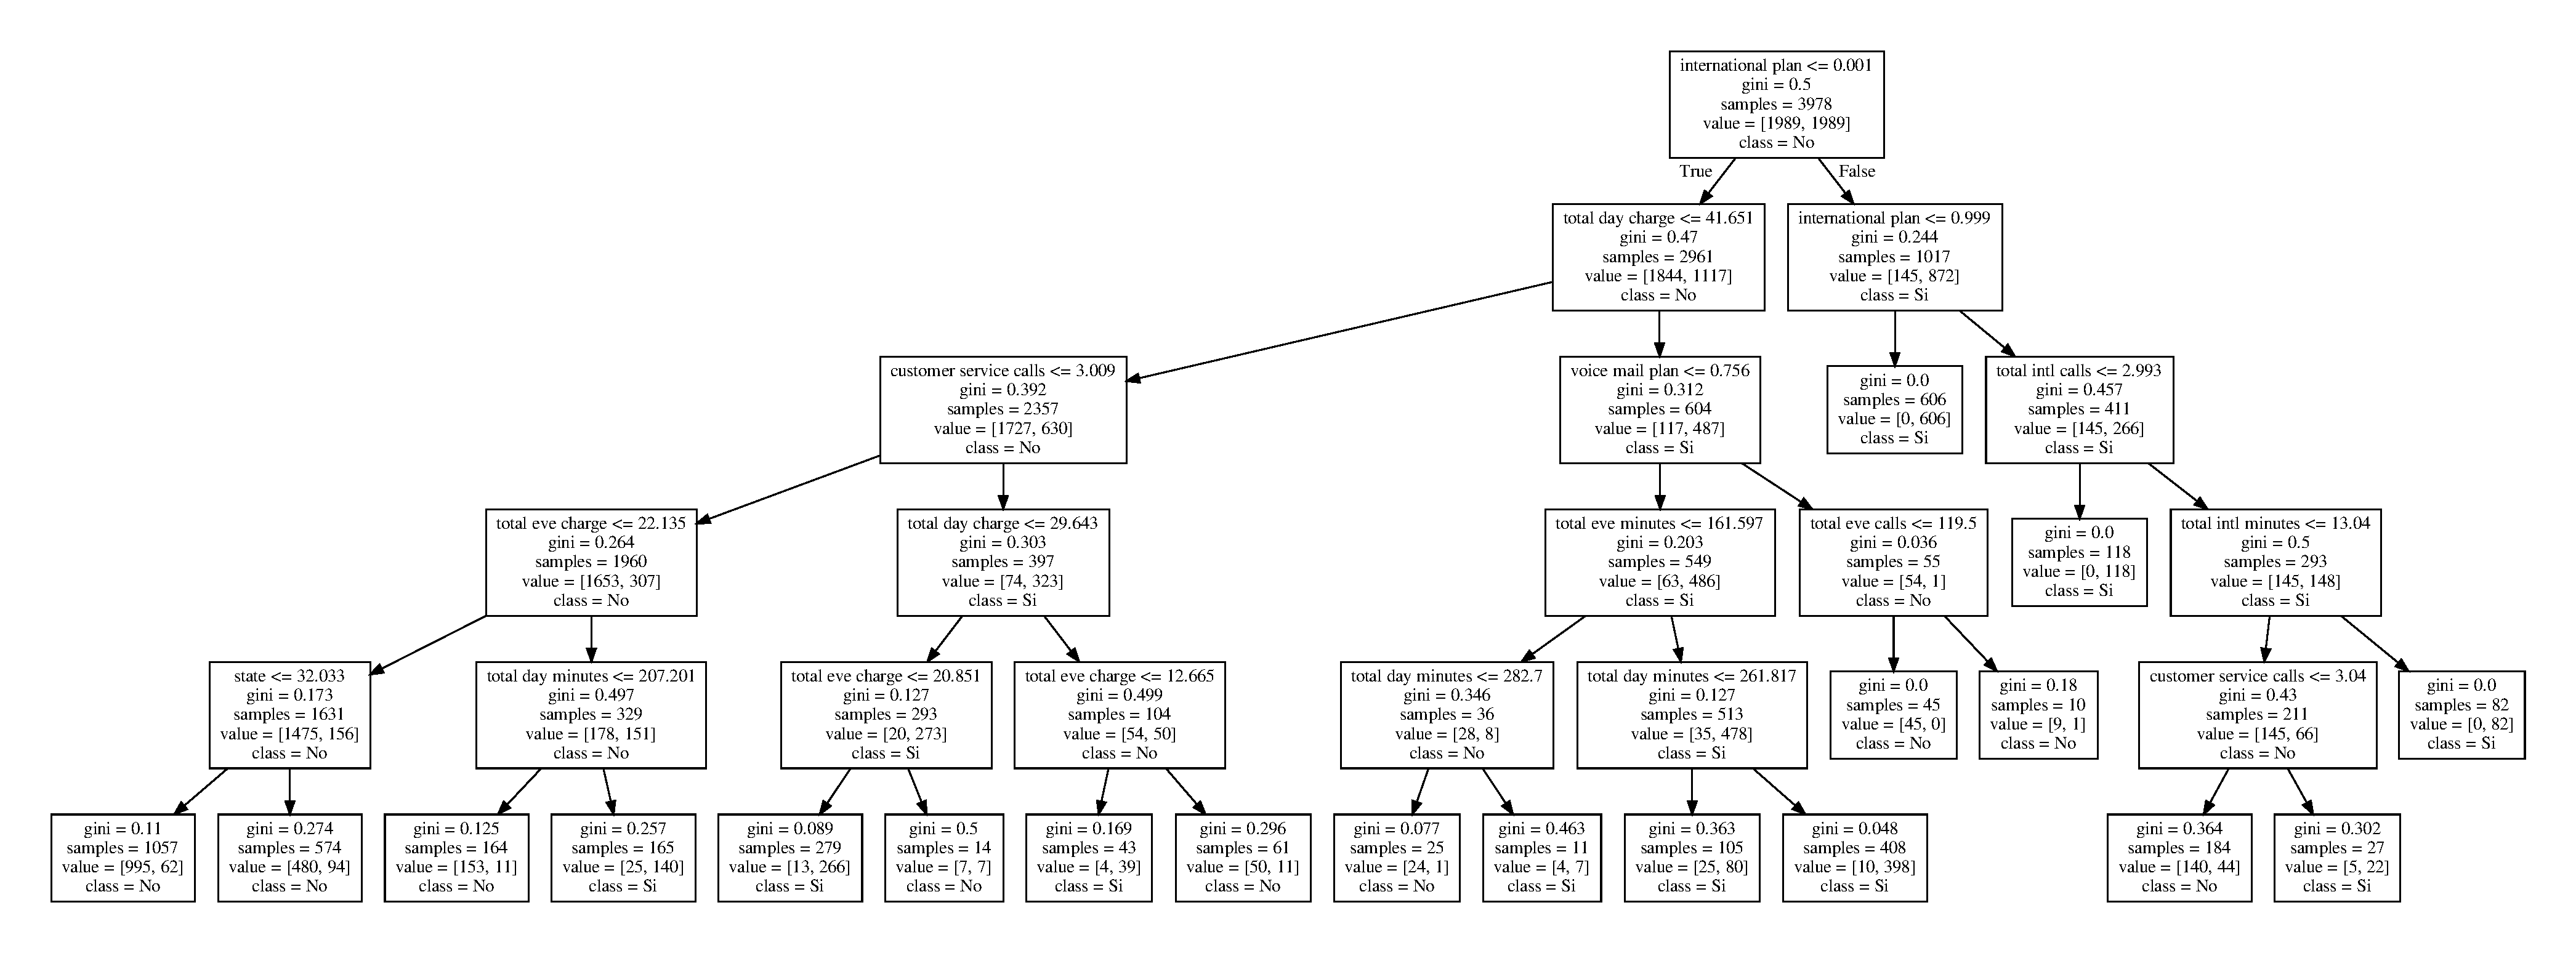
\includegraphics[width=0.5\textwidth]{Tree}			
		  	\end{figure}
		  	Para clasificar una instancia desconocida se recorre el �rbol de arriba hacia abajo de acuerdo a los valores de los atributos probados en cada nodo y cuando se llega a una hoja, la instancia se clasifica con la clase indicada por esa hoja.
		  	\vspace{1cm}
		  	
		  	De forma general, el 93.1\% de los datos el modelo los clasificar� correctamente.$$accuracy=0.9310$$ adem�s, el modelo tiene una precisi�n del 87\% al momento de predecir a un usuario como desertor. $$precision=0.87$$		
\end{document}